\chapter{Overview}

Zubax Komar is a high-end FOC ESC based on the \text{T\'elega} motor control technology.
Komar is designed for use in propulsion systems of light unmanned aerial (UAV), underwater, and surface vehicles.
The controller provides up to 2500 W\footnote{Forced air cooling is assumed}
of continuous power output and supports a wide range of operating voltages
12 -- 51 V (4 -- 12S $\text{LiCoO}_\text{2}$ battery).
The device is a highly tunable controller and can be fine-tuned for any motor-propeller combination
for optimal dynamic response.
Zubax Komar offers several control modes that make it suitable for application in a wide range of propulsion systems.
Komar is fully UAVCAN compatible and enables easy integration into the end system by using a full set
of standard UAVCAN Micro connectors\footnote{For more details refer to
\url{https://uavcan.org/Specification/8._Hardware_design_recommendations/}} (two connectors per CAN interface).
The device constantly measures and reports all the crucial variables during operation
(e.g. its own temperature, motor temperature, current consumption, battery voltage, etc.)
improving system reliability.

\section{System integration}
Zubax Komar is a single supply device, which means that the device does not expose any power supply inputs except
for the high power supply. The 5 V rails of the CAN interfaces are not used by the device;
rather, the device may provide 5 V power line for UAVCAN bus from its internal DC-DC converter if needed.

\begin{figure}[h]
    \centering
    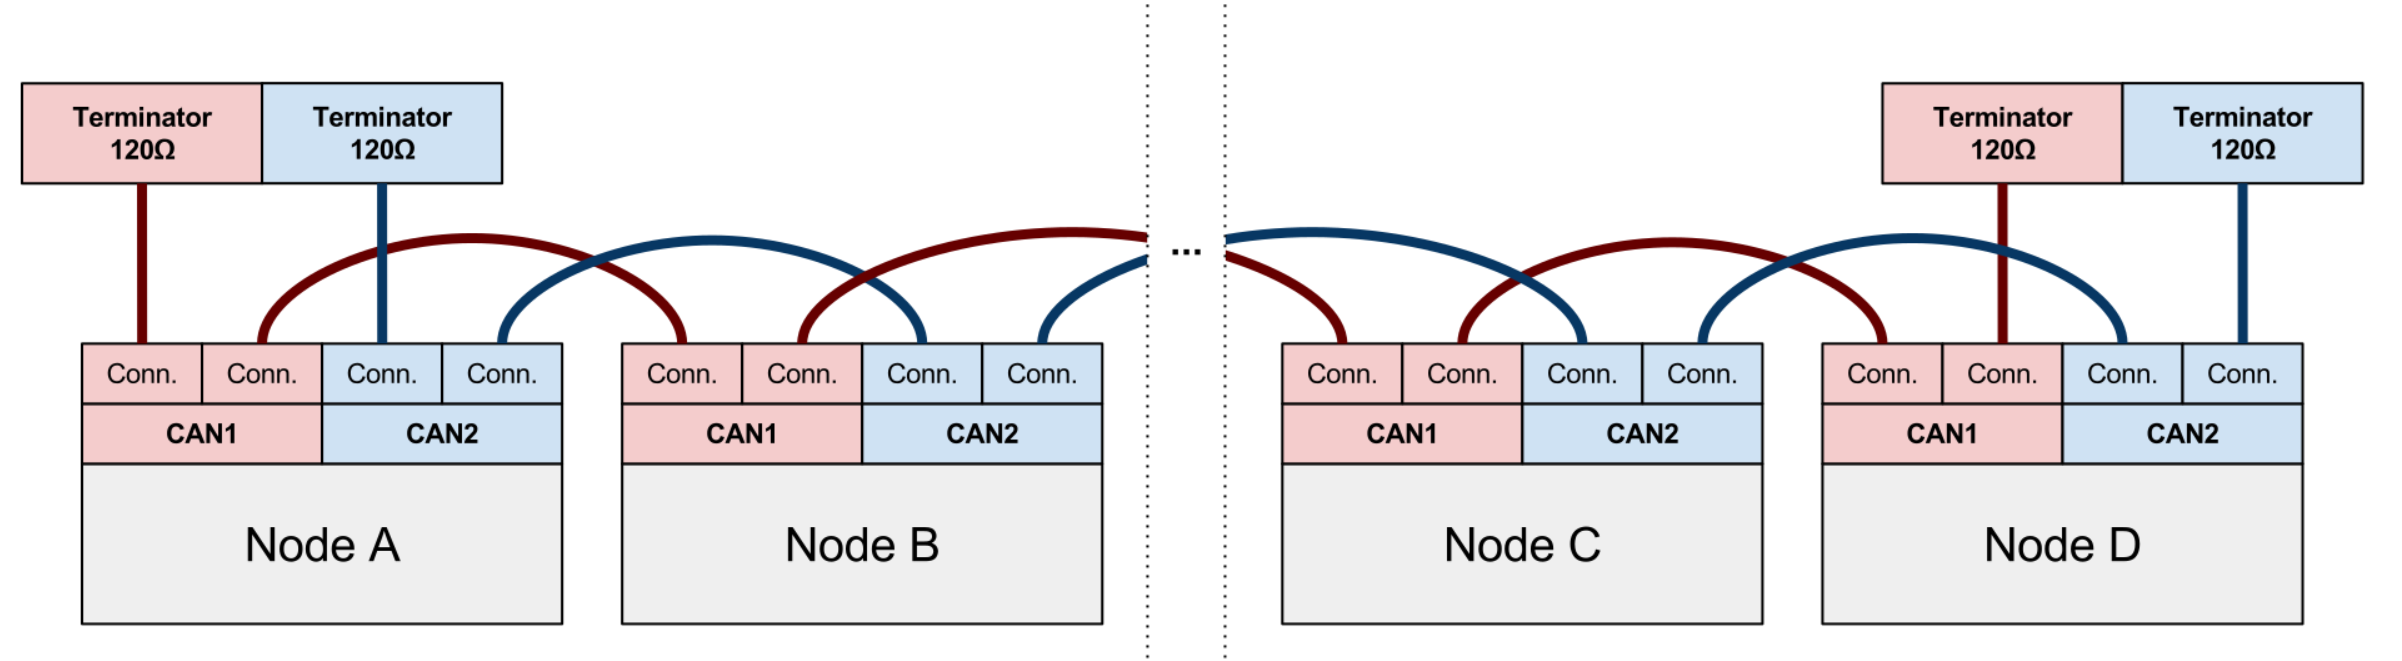
\includegraphics[width=1\textwidth]{can_intergration.png}
    \caption{Connection of CAN nodes}
\end{figure}
